
\section{Figures}\label{App:Figures}

\subsection{Excluded consumer data sets}\label{App:Figures:Excluded}

\begin{centering}
\begin{figure}[!htbp]
        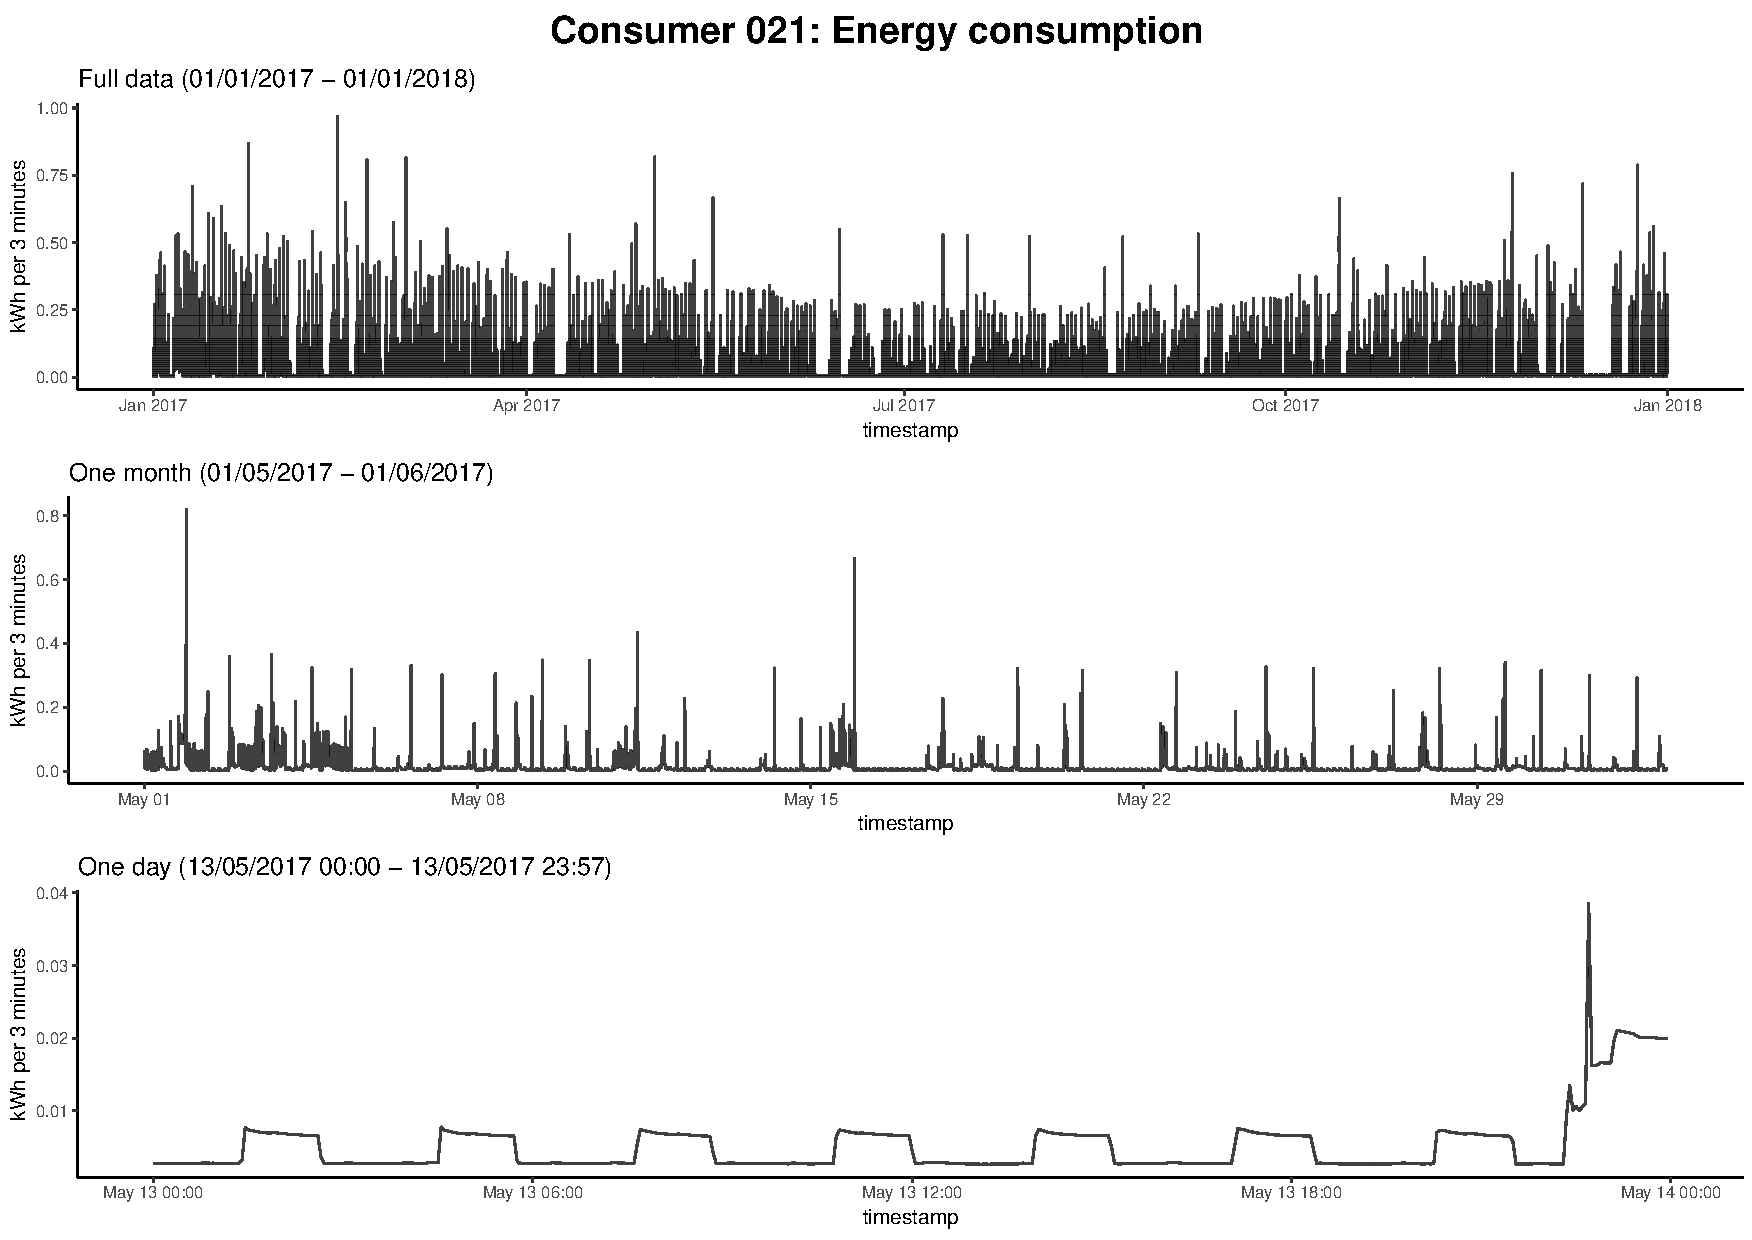
\includegraphics[width=\textwidth-0.85cm]{thesis/graphs/timeseries/c021_cons.pdf}\vspace{0.3cm}
        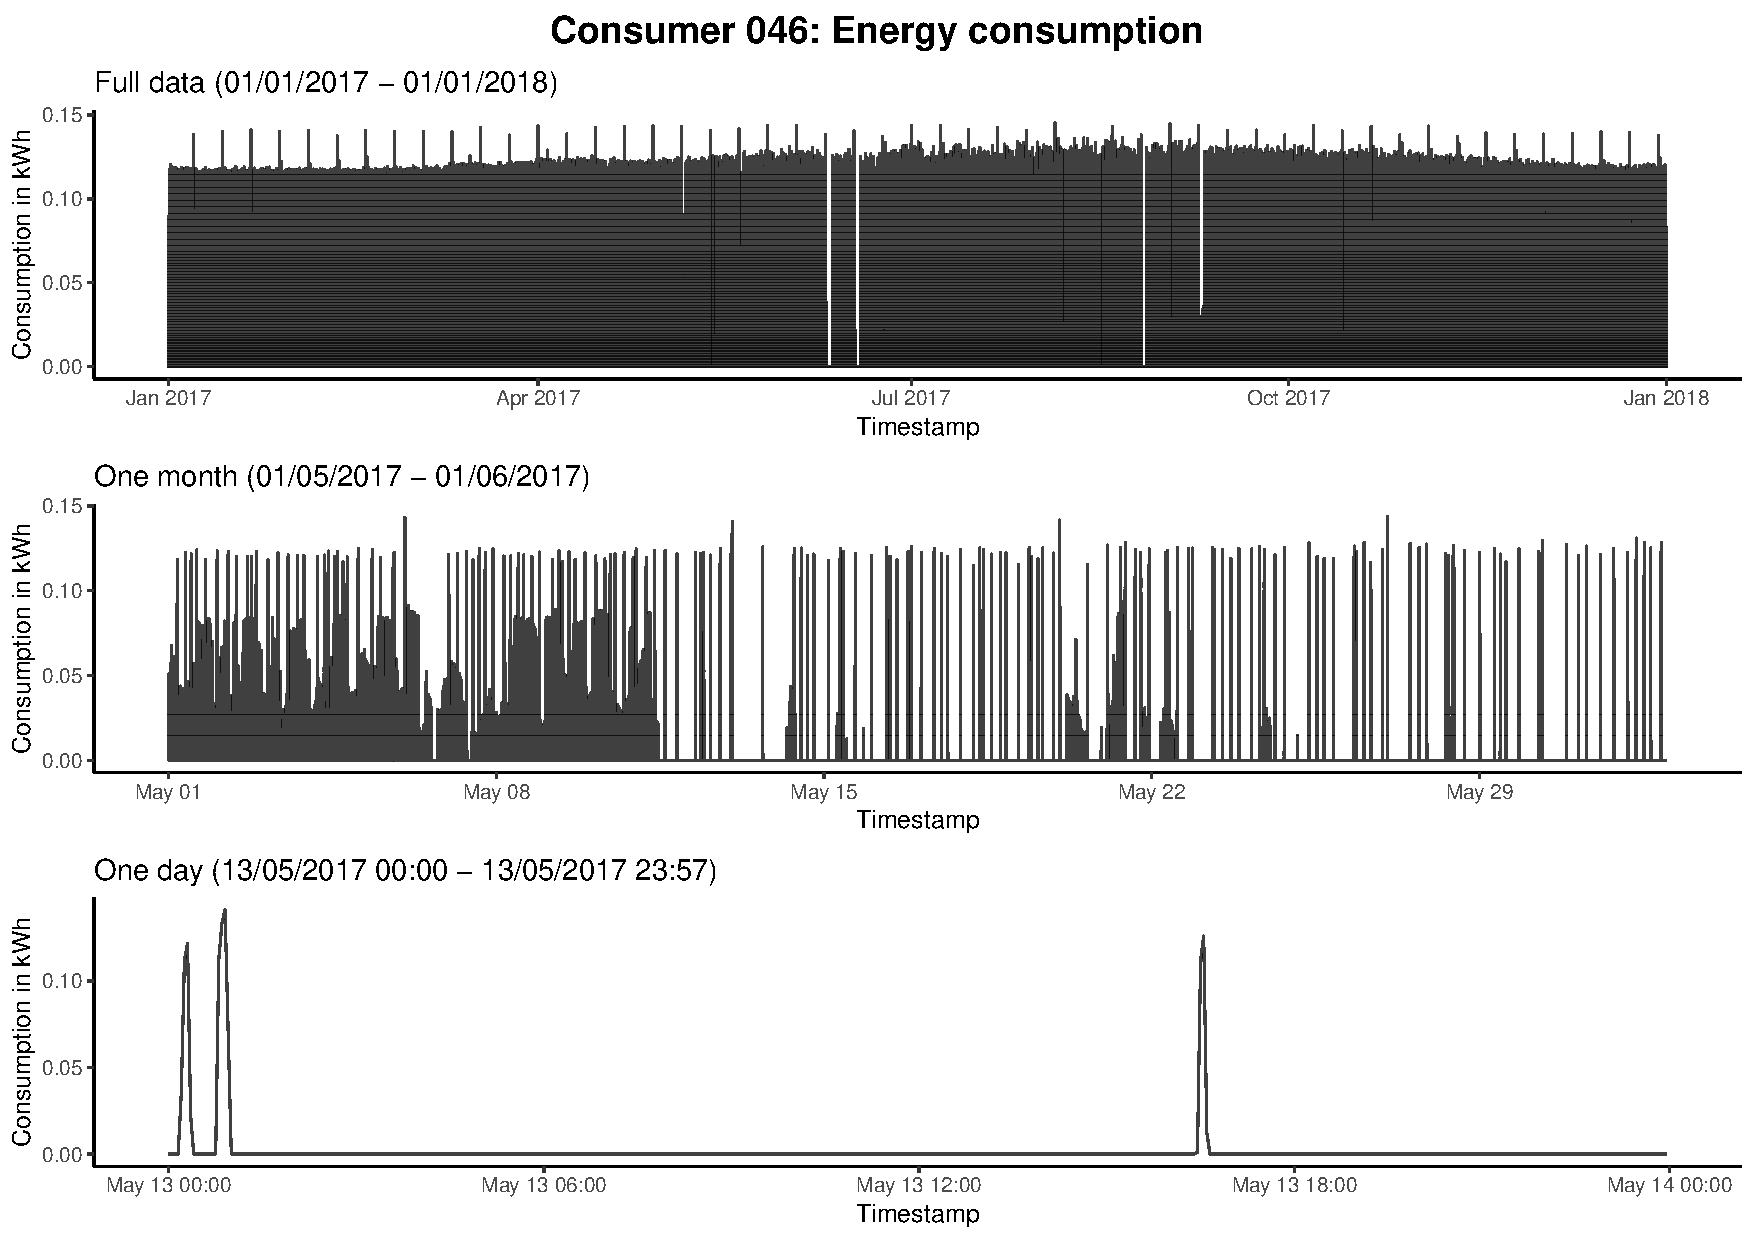
\includegraphics[width=\textwidth-0.85cm]{thesis/graphs/timeseries/c046_cons.pdf}
\end{figure}
\begin{figure}[!htbp]
        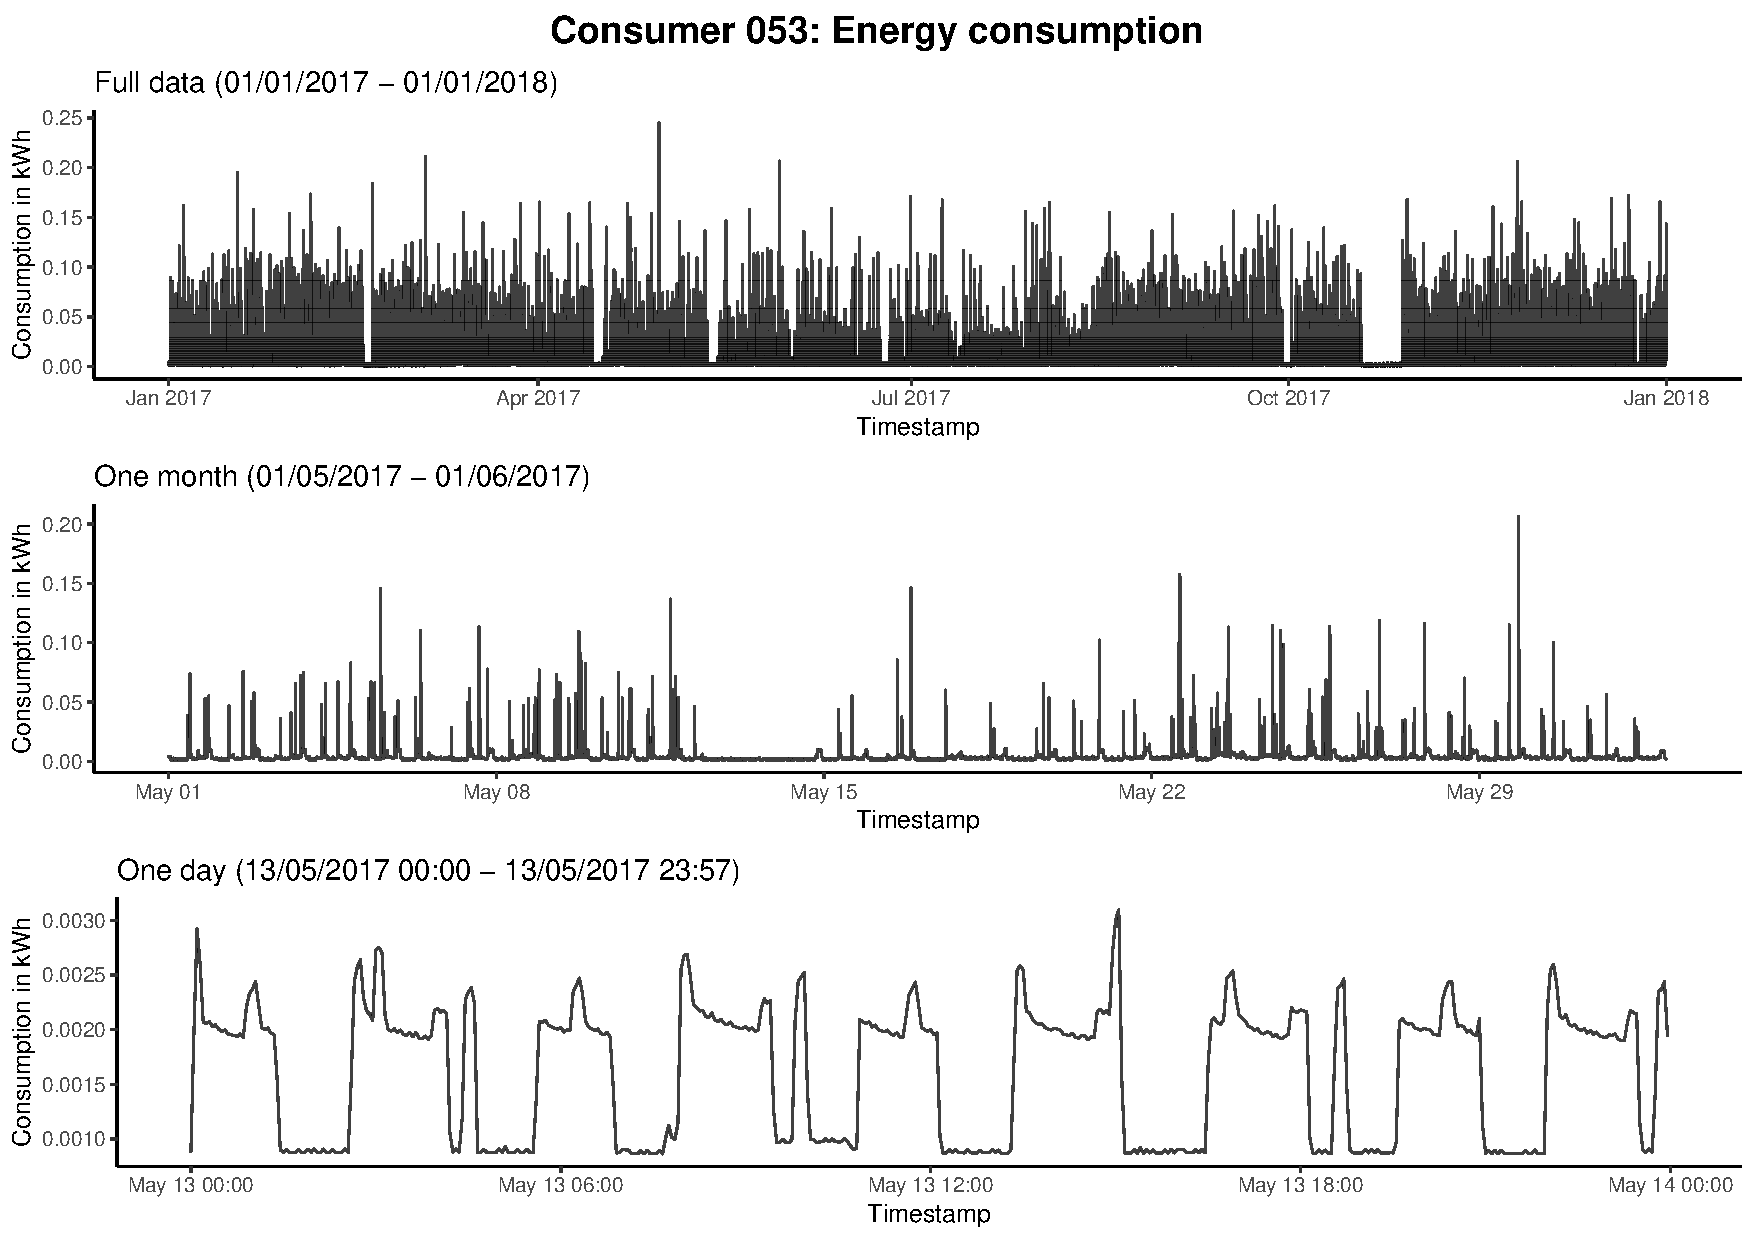
\includegraphics[width=\textwidth-0.85cm]{thesis/graphs/timeseries/c053_cons.pdf}\vspace{0.3cm}
        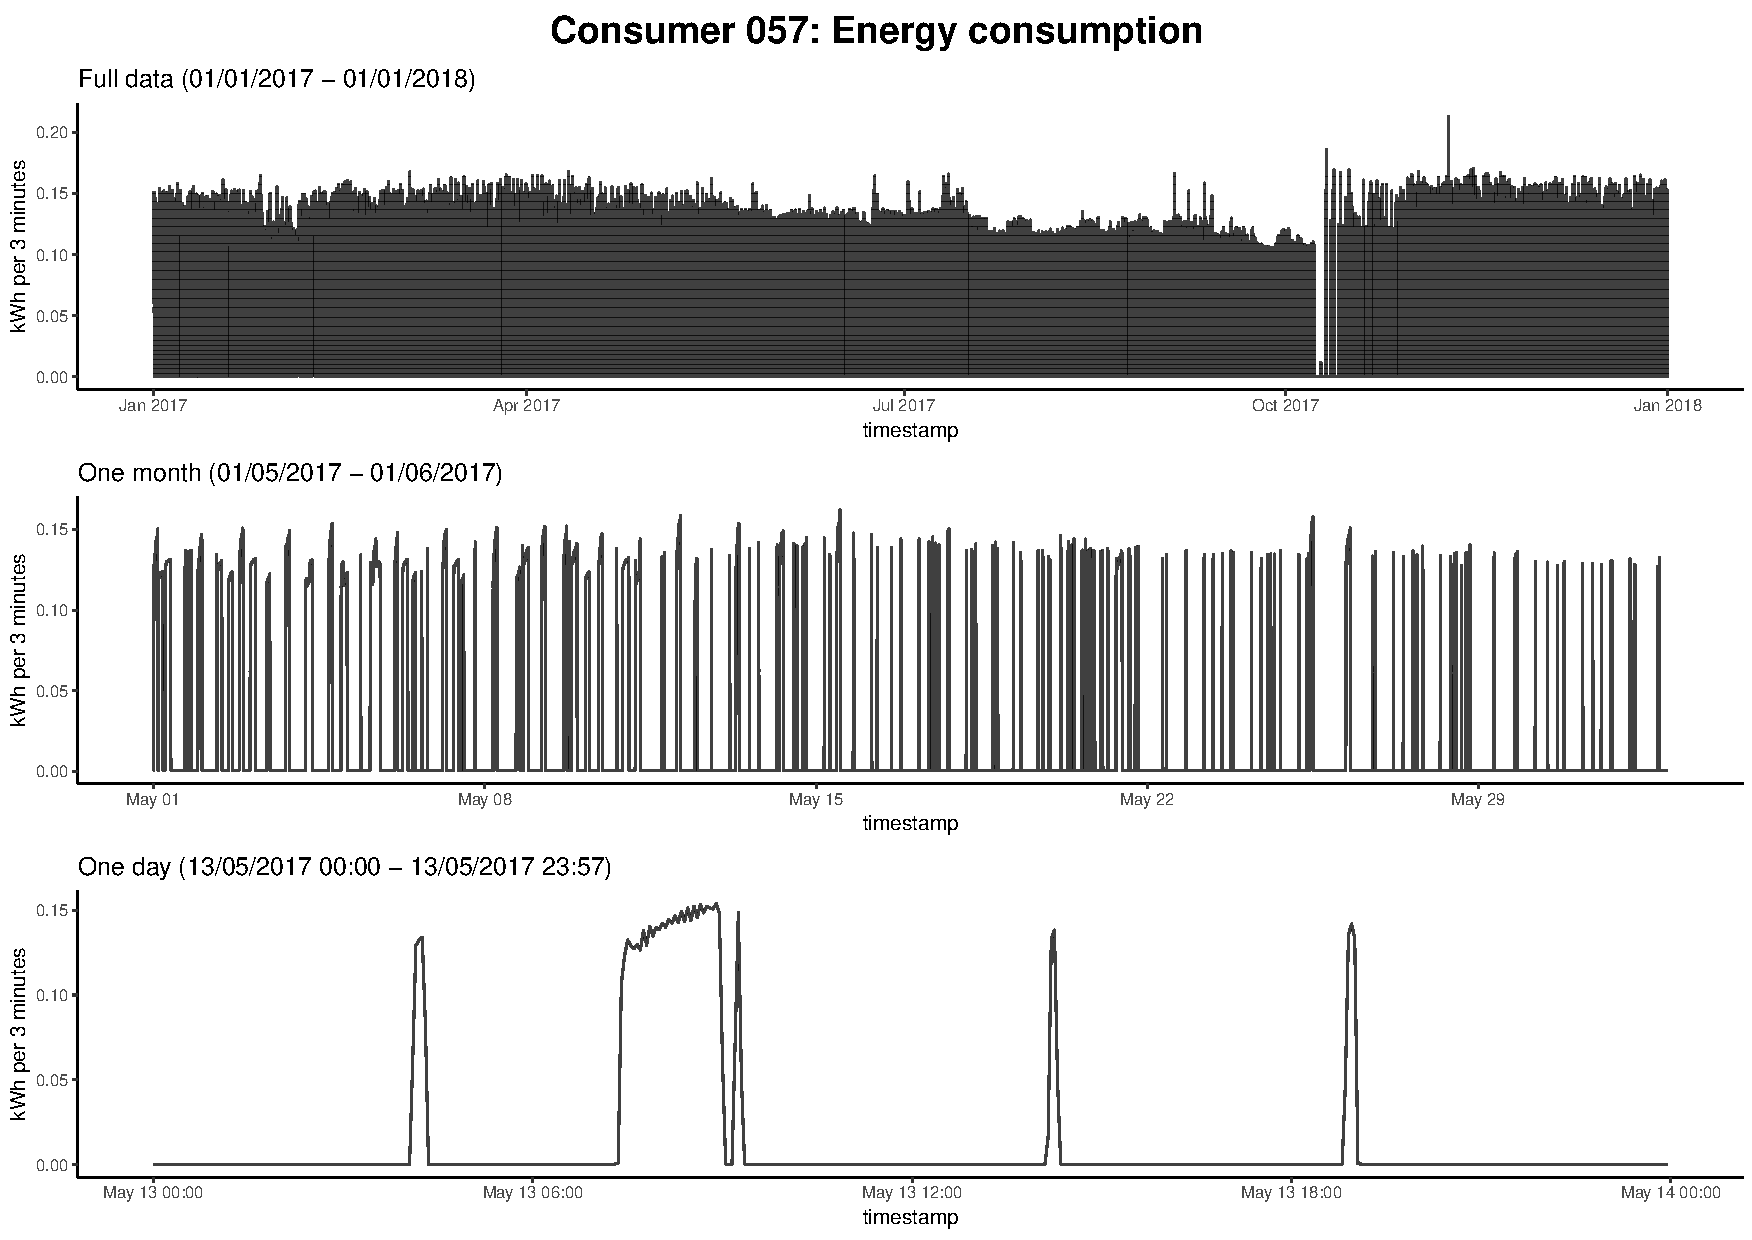
\includegraphics[width=\textwidth-0.85cm]{thesis/graphs/timeseries/c057_cons.pdf}
\end{figure}
\begin{figure}[!htbp]
        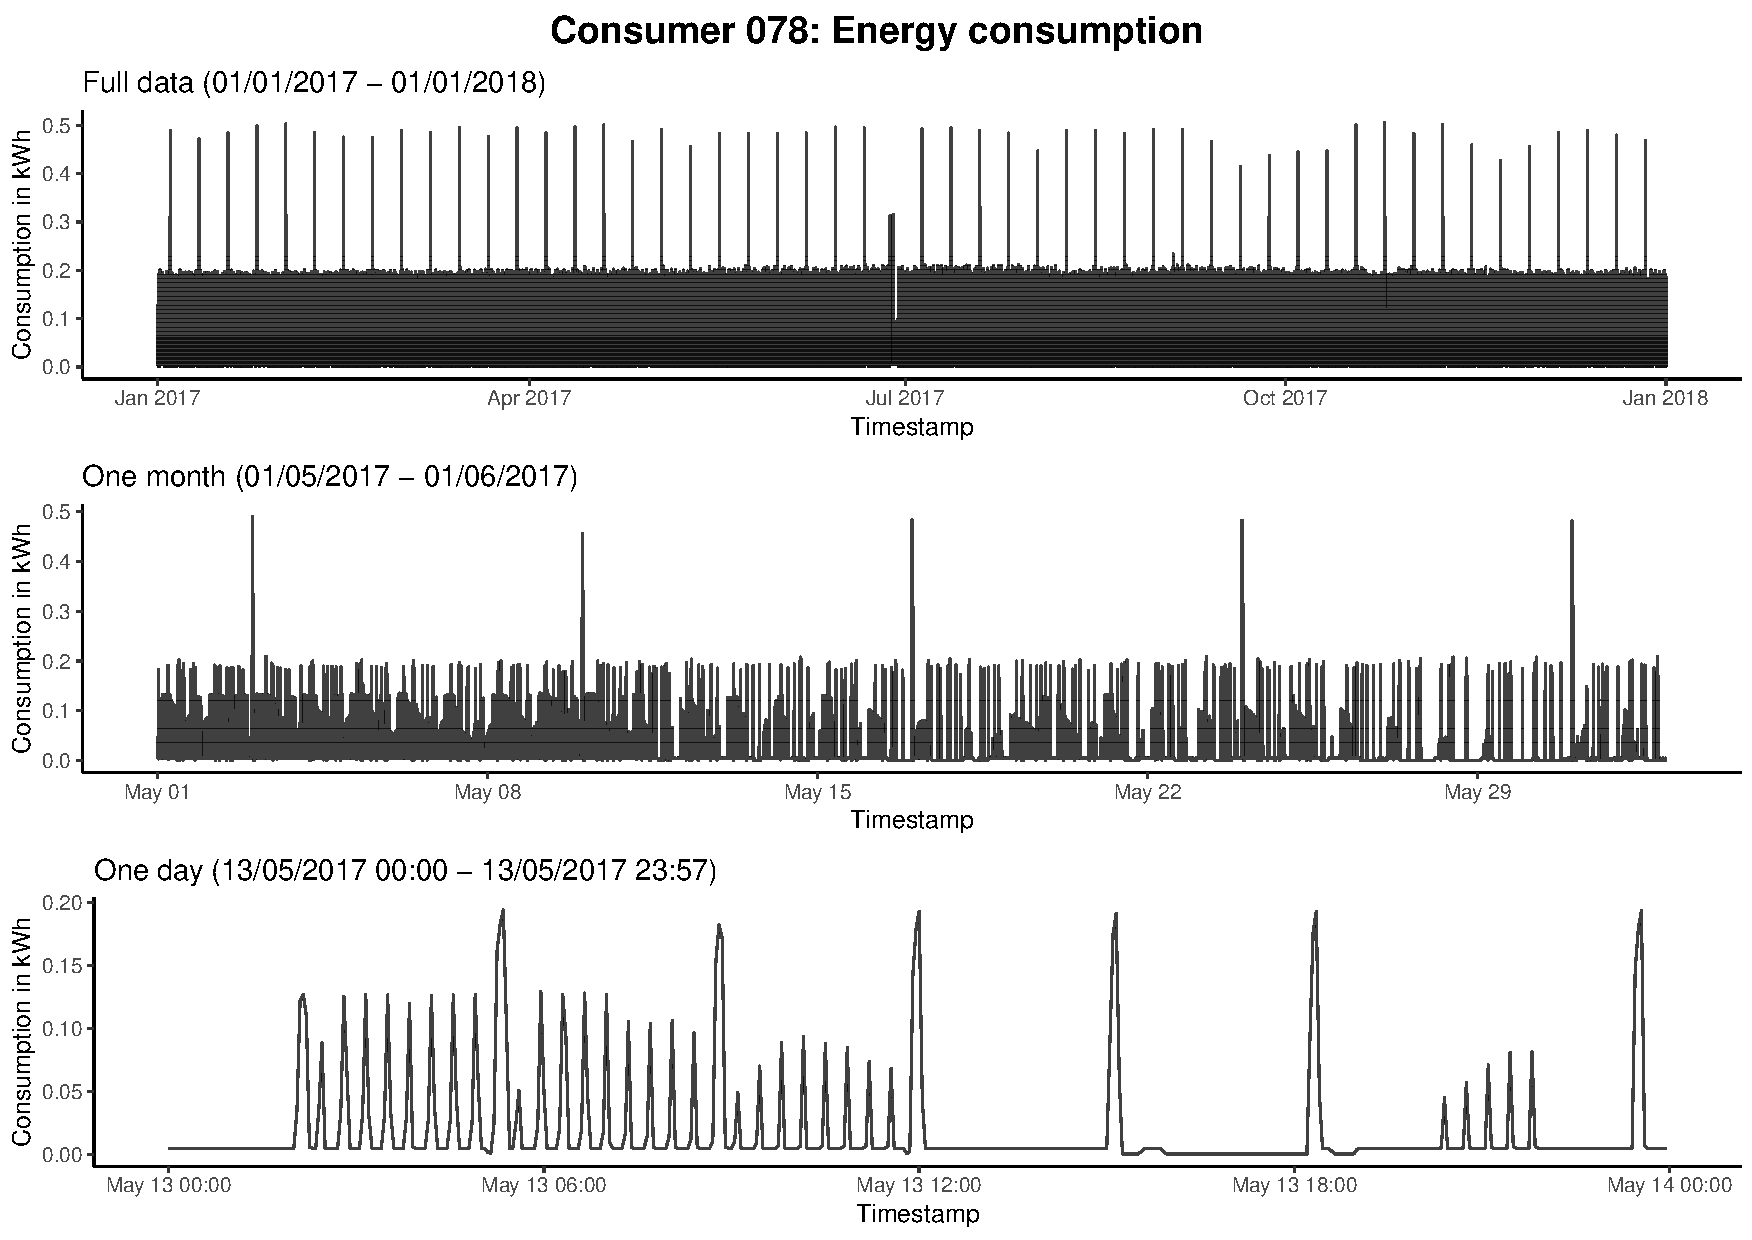
\includegraphics[width=\textwidth-0.85cm]{thesis/graphs/timeseries/c078_cons.pdf}\vspace{0.3cm}
        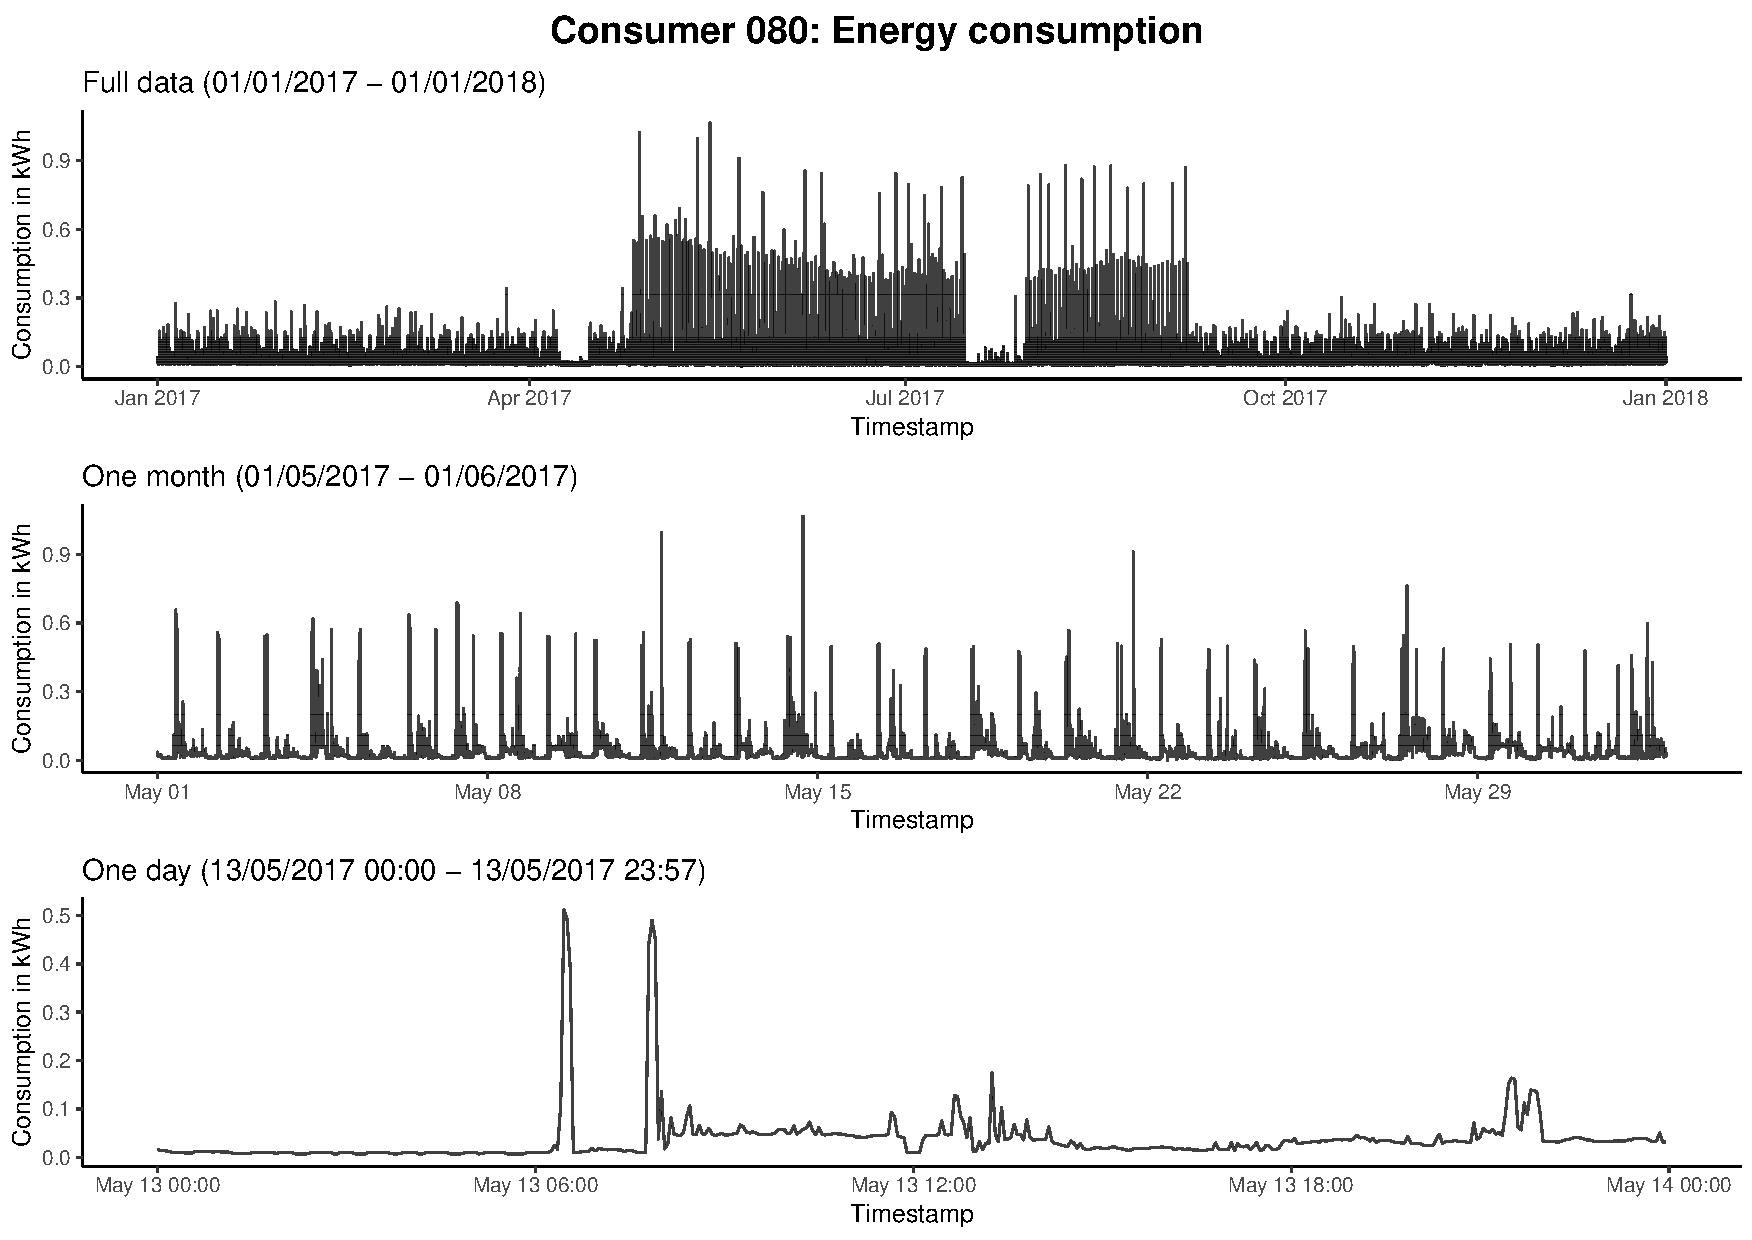
\includegraphics[width=\textwidth-0.85cm]{thesis/graphs/timeseries/c080_cons.pdf}
        \caption[Consumer data sets excluded due to peculiarities in the consumption patterns]{Consumer data sets excluded due to peculiarities in the consumption patterns. \quantnet}
        \label{App:Fig:excludedcons}
\end{figure}
\end{centering}


%%%%%%%%%%%%%%%%%%%%%%%%%%%%%%%%%%%%%%%%%%%%%%%%%%%%%%%%%%%%

\begin{figure}[ht]
    \begin{center}
        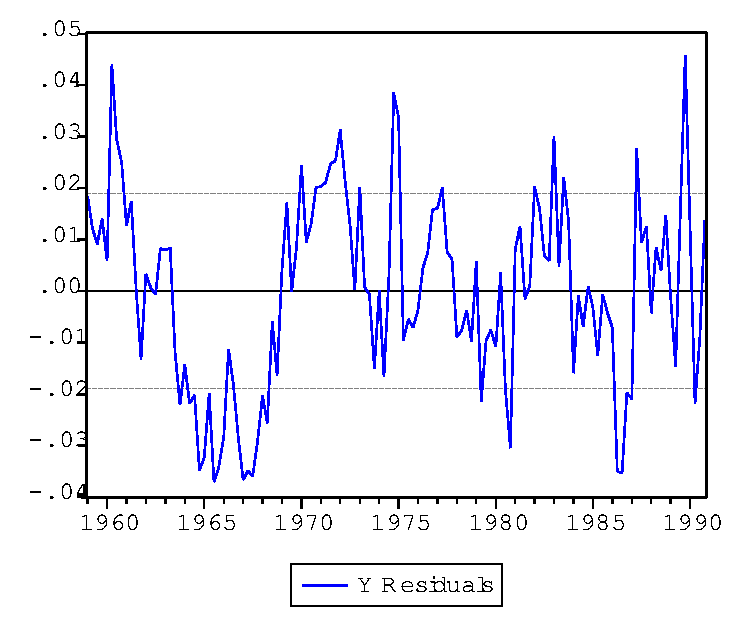
\includegraphics[scale=0.5,angle=0]{thesis/figures/graph.pdf}
        \caption{Estimated residuals (2) from model XXX. ...}
        \label{Fig:Resids2}
    \end{center}
\end{figure}
